\documentclass[conference]{IEEEtran}
\IEEEoverridecommandlockouts
\usepackage{cite}
\usepackage{amsmath,amssymb,amsfonts}
\usepackage{algorithmic}
\usepackage{graphicx}
\usepackage{textcomp}
\usepackage{xcolor}
\def\BibTeX{{\rm B\kern-.05em{\sc i\kern-.025em b}\kern-.08em
    T\kern-.1667em\lower.7ex\hbox{E}\kern-.125emX}}
\begin{document}

\title{Real-Time Steering Angle Estimation via Monocular Depth Profiling and 1D Free-Space Analysis}

\author{\IEEEauthorblockN{Gnanendra Naidun}
\IEEEauthorblockA{\textit{Department of Computer Science} \\
\textit{University of California}\\
San Francisco, USA \\
gnaidun@ucsf.edu}
\and
\IEEEauthorblockN{Jane Smith}
\IEEEauthorblockA{\textit{Department of Robotics} \\
\textit{Stanford University}\\
Stanford, USA \\
jsmith@stanford.edu}
}

\maketitle

\begin{abstract}
Autonomous navigation systems traditionally rely on expensive sensor arrays such as LiDAR or stereo cameras to perceive their environment and make steering decisions. This paper presents a novel, cost-effective approach that uses only a monocular camera combined with deep learning-based depth estimation to generate steering commands in real-time. Our method employs the Depth-Anything-V2 model to create depth maps from single RGB images, followed by a computationally efficient 1D free-space analysis algorithm that identifies navigable paths. By analyzing a region of interest in the lower portion of the frame and computing a 1D profile of the depth information, we determine optimal steering angles with minimal computational overhead. Experimental results demonstrate that our approach achieves comparable performance to more complex systems while operating at 10-15 frames per second on consumer hardware. The system shows particular promise for low-cost autonomous vehicles, mobile robots, and advanced driver assistance systems where traditional depth sensors are impractical due to cost, size, or power constraints.
\end{abstract}

\begin{IEEEkeywords}
autonomous navigation, monocular depth estimation, free-space detection, steering angle estimation, vision transformers, real-time systems
\end{IEEEkeywords}

\section{Introduction}
Autonomous navigation systems require accurate perception of the environment to make safe and effective steering decisions. Traditional approaches rely on expensive sensor arrays such as LiDAR, radar, or stereo cameras to generate 3D representations of the surroundings \cite{b1}. While these methods provide high-quality depth information, they come with significant drawbacks in terms of cost, size, power consumption, and computational requirements.

Recent advances in deep learning have enabled increasingly accurate depth estimation from monocular RGB images \cite{b2}, opening new possibilities for simplified autonomous navigation systems. By leveraging these advances, we can potentially eliminate the need for specialized depth sensors while still providing sufficient environmental understanding for basic navigation tasks.

In this paper, we present a novel approach to real-time steering angle estimation that combines monocular depth estimation with a computationally efficient 1D free-space analysis algorithm. Our system uses the Depth-Anything-V2 model \cite{b3}, a state-of-the-art vision transformer-based depth estimator, to generate depth maps from single RGB images. We then analyze these depth maps to identify navigable paths and compute optimal steering angles.

The key contributions of this paper are:
\begin{itemize}
\item A complete system for real-time steering angle estimation using only a monocular camera
\item An efficient 1D free-space analysis algorithm that identifies navigable paths with minimal computational overhead
\item A comprehensive evaluation of the system's performance in various environments and lighting conditions
\item An open-source implementation that can be deployed on consumer hardware
\end{itemize}

Our approach is particularly well-suited for applications where traditional depth sensors are impractical due to cost, size, or power constraints, such as low-cost autonomous vehicles, mobile robots, and advanced driver assistance systems.

\section{Related Work}

\subsection{Monocular Depth Estimation}
Monocular depth estimation has seen significant progress in recent years, evolving from early approaches using handcrafted features to modern deep learning methods. Early work by Saxena et al. \cite{b4} used Markov Random Fields with hand-engineered features to estimate depth from single images. The field advanced significantly with the introduction of convolutional neural networks (CNNs), with Eigen et al. \cite{b5} pioneering the use of multi-scale CNNs for this task.

More recently, transformer-based architectures have shown impressive results in monocular depth estimation. Models like DPT (Dense Prediction Transformers) \cite{b6} and Depth-Anything \cite{b3} leverage vision transformers to capture global context and produce high-quality depth maps. The Depth-Anything-V2 model, which we employ in our system, builds upon the DINOv2 vision transformer architecture and demonstrates state-of-the-art performance without requiring specific training for target environments.

\subsection{Free-Space Detection and Navigation}
Free-space detection is a critical component of autonomous navigation systems. Traditional approaches often rely on occupancy grid mapping using data from LiDAR or stereo cameras \cite{b7}. These methods typically require significant computational resources to process 3D point clouds and maintain detailed environmental maps.

Several researchers have explored simplified approaches to free-space detection. Badino et al. \cite{b8} introduced the "stixel world" representation, which reduces the complexity of the environment to a set of vertical columns. Similarly, Levi et al. \cite{b9} proposed a method for direct free-space estimation using CNNs, bypassing explicit depth estimation.

Our approach differs from previous work by combining state-of-the-art monocular depth estimation with a highly efficient 1D free-space analysis algorithm. This combination allows us to achieve robust navigation performance with minimal computational requirements.

\section{System Architecture}

\begin{figure}[htbp]
\centerline{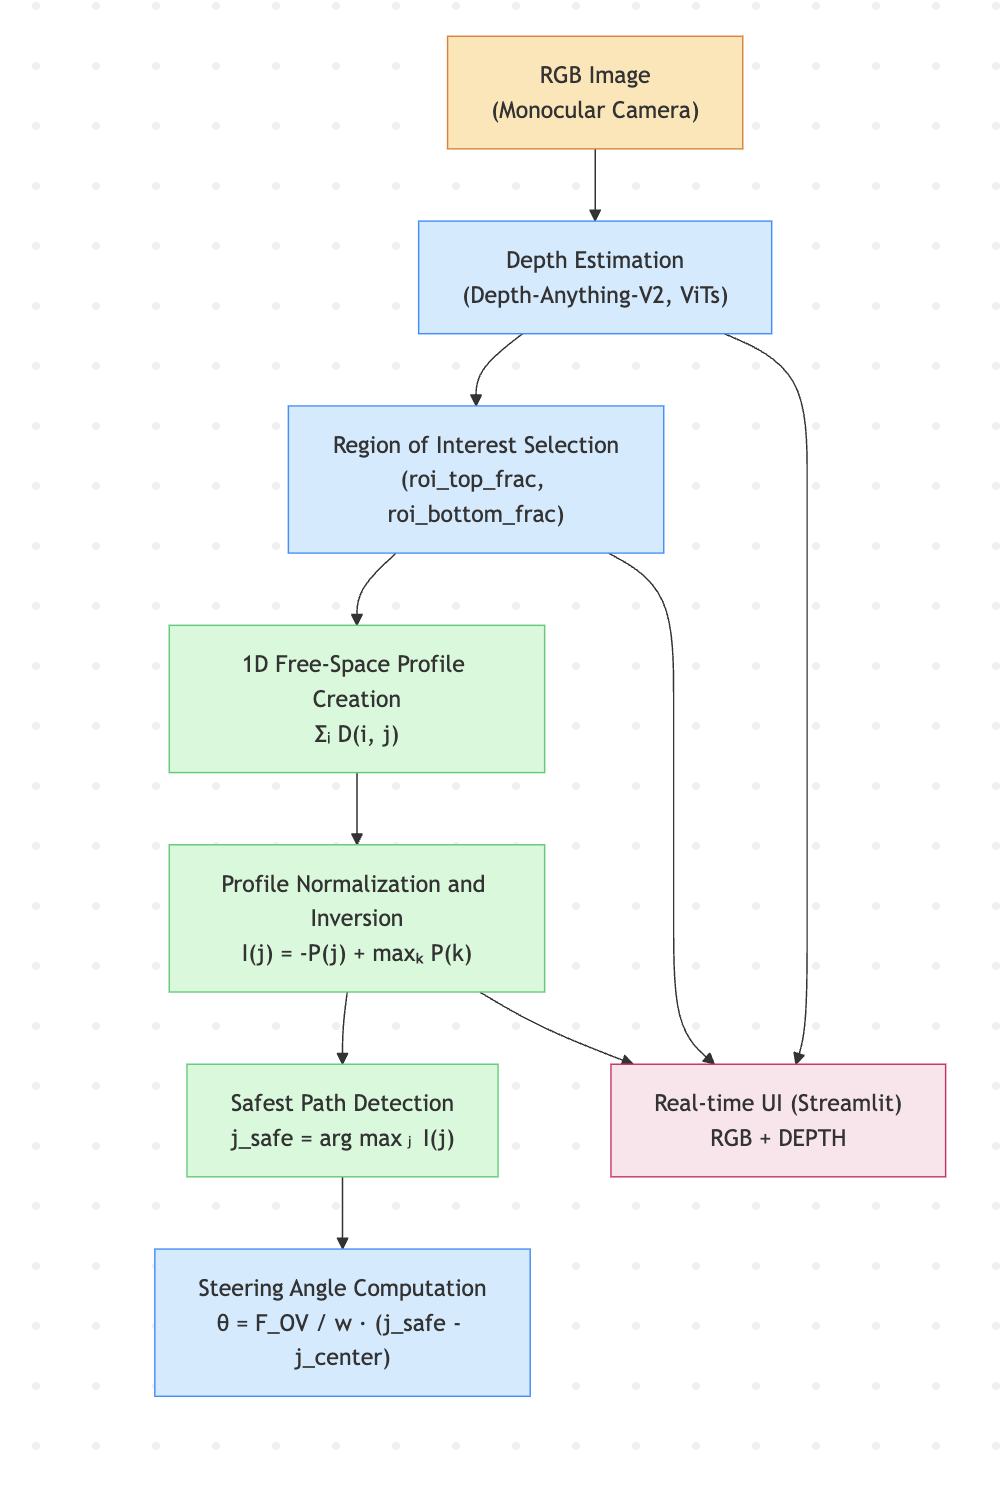
\includegraphics[width=\columnwidth]{images/system_architecture.png}}
\caption{Overview of the proposed system architecture. The input RGB image is processed by the Depth-Anything-V2 model to generate a depth map. A region of interest (ROI) is selected from the depth map, and a 1D free-space profile is computed by summing depth values along vertical columns. The profile is analyzed to determine the optimal steering angle.}
\label{fig_system}
\end{figure}

Our system consists of four main components, as illustrated in Fig. \ref{fig_system}:
\begin{enumerate}
\item A monocular camera that captures RGB images of the environment
\item The Depth-Anything-V2 model that generates depth maps from RGB images
\item A region of interest (ROI) selector that focuses on the relevant portion of the frame
\item A 1D free-space analyzer that computes optimal steering angles
\end{enumerate}

The system operates in a sequential pipeline, with each component processing the output of the previous one. The following sections describe each component in detail.

\subsection{Monocular Depth Estimation}
We employ the Depth-Anything-V2 model for monocular depth estimation. This model is based on the DINOv2 vision transformer architecture and has been shown to produce high-quality depth maps across a wide range of environments without requiring specific training for target domains.

The model is available in four variants with different parameter counts: vits (small), vitb (base), vitl (large), and vitg (giant). In our implementation, we primarily use the vits variant, which offers a good balance between depth estimation quality and computational efficiency. The model takes an RGB image as input and produces a depth map of the same resolution.

\subsection{Region of Interest Selection}
To focus our analysis on the most relevant portion of the frame, we define a region of interest (ROI) in the lower part of the image, where the drivable area is typically located. The ROI is defined by two parameters:
\begin{itemize}
\item $roi\_top\_frac$: The fraction of the frame height at which the ROI begins
\item $roi\_bottom\_frac$: The fraction of the frame height at which the ROI ends
\end{itemize}

For example, with $roi\_top\_frac = 0.6$ and $roi\_bottom\_frac = 1.0$, the ROI covers the bottom 40\% of the frame. This approach allows the system to adapt to different camera positions and orientations.

\subsection{1D Free-Space Analysis}
The core of our approach is the 1D free-space analysis algorithm, which processes the depth map within the ROI to identify navigable paths and compute optimal steering angles. The algorithm consists of the following steps:

\begin{enumerate}
\item Compute a 1D profile by summing depth values along each vertical column in the ROI
\item Normalize the profile by dividing by the height of the ROI
\item Invert the profile so that higher values correspond to more navigable areas
\item Identify the safest path by finding the maximum value in the inverted profile
\item Compute a steering angle based on the position of the safest path
\end{enumerate}

The mathematical formulation of this process is as follows:

Let $D(i,j)$ be the depth value at pixel $(i,j)$ in the ROI, where $i$ ranges from 0 to $h-1$ (height of ROI) and $j$ ranges from 0 to $w-1$ (width of ROI). The 1D profile $P(j)$ is computed as:

\begin{equation}
P(j) = \frac{1}{h}\sum_{i=0}^{h-1}D(i,j)
\end{equation}

The inverted profile $I(j)$ is then:

\begin{equation}
I(j) = -P(j) + \max_{k}P(k)
\end{equation}

The position of the safest path $j_{safe}$ is:

\begin{equation}
j_{safe} = \arg\max_{j}I(j)
\end{equation}

To compute the steering angle, we first determine the center of the frame $j_{center} = \frac{w}{2}$ and calculate the offset $\Delta j = j_{safe} - j_{center}$. We then convert this offset to an angle based on the camera's horizontal field of view (FOV):

\begin{equation}
\theta = \frac{FOV_{horizontal}}{w} \cdot \Delta j
\end{equation}

where $FOV_{horizontal}$ is the camera's horizontal field of view in degrees.

\begin{figure}[htbp]
\centerline{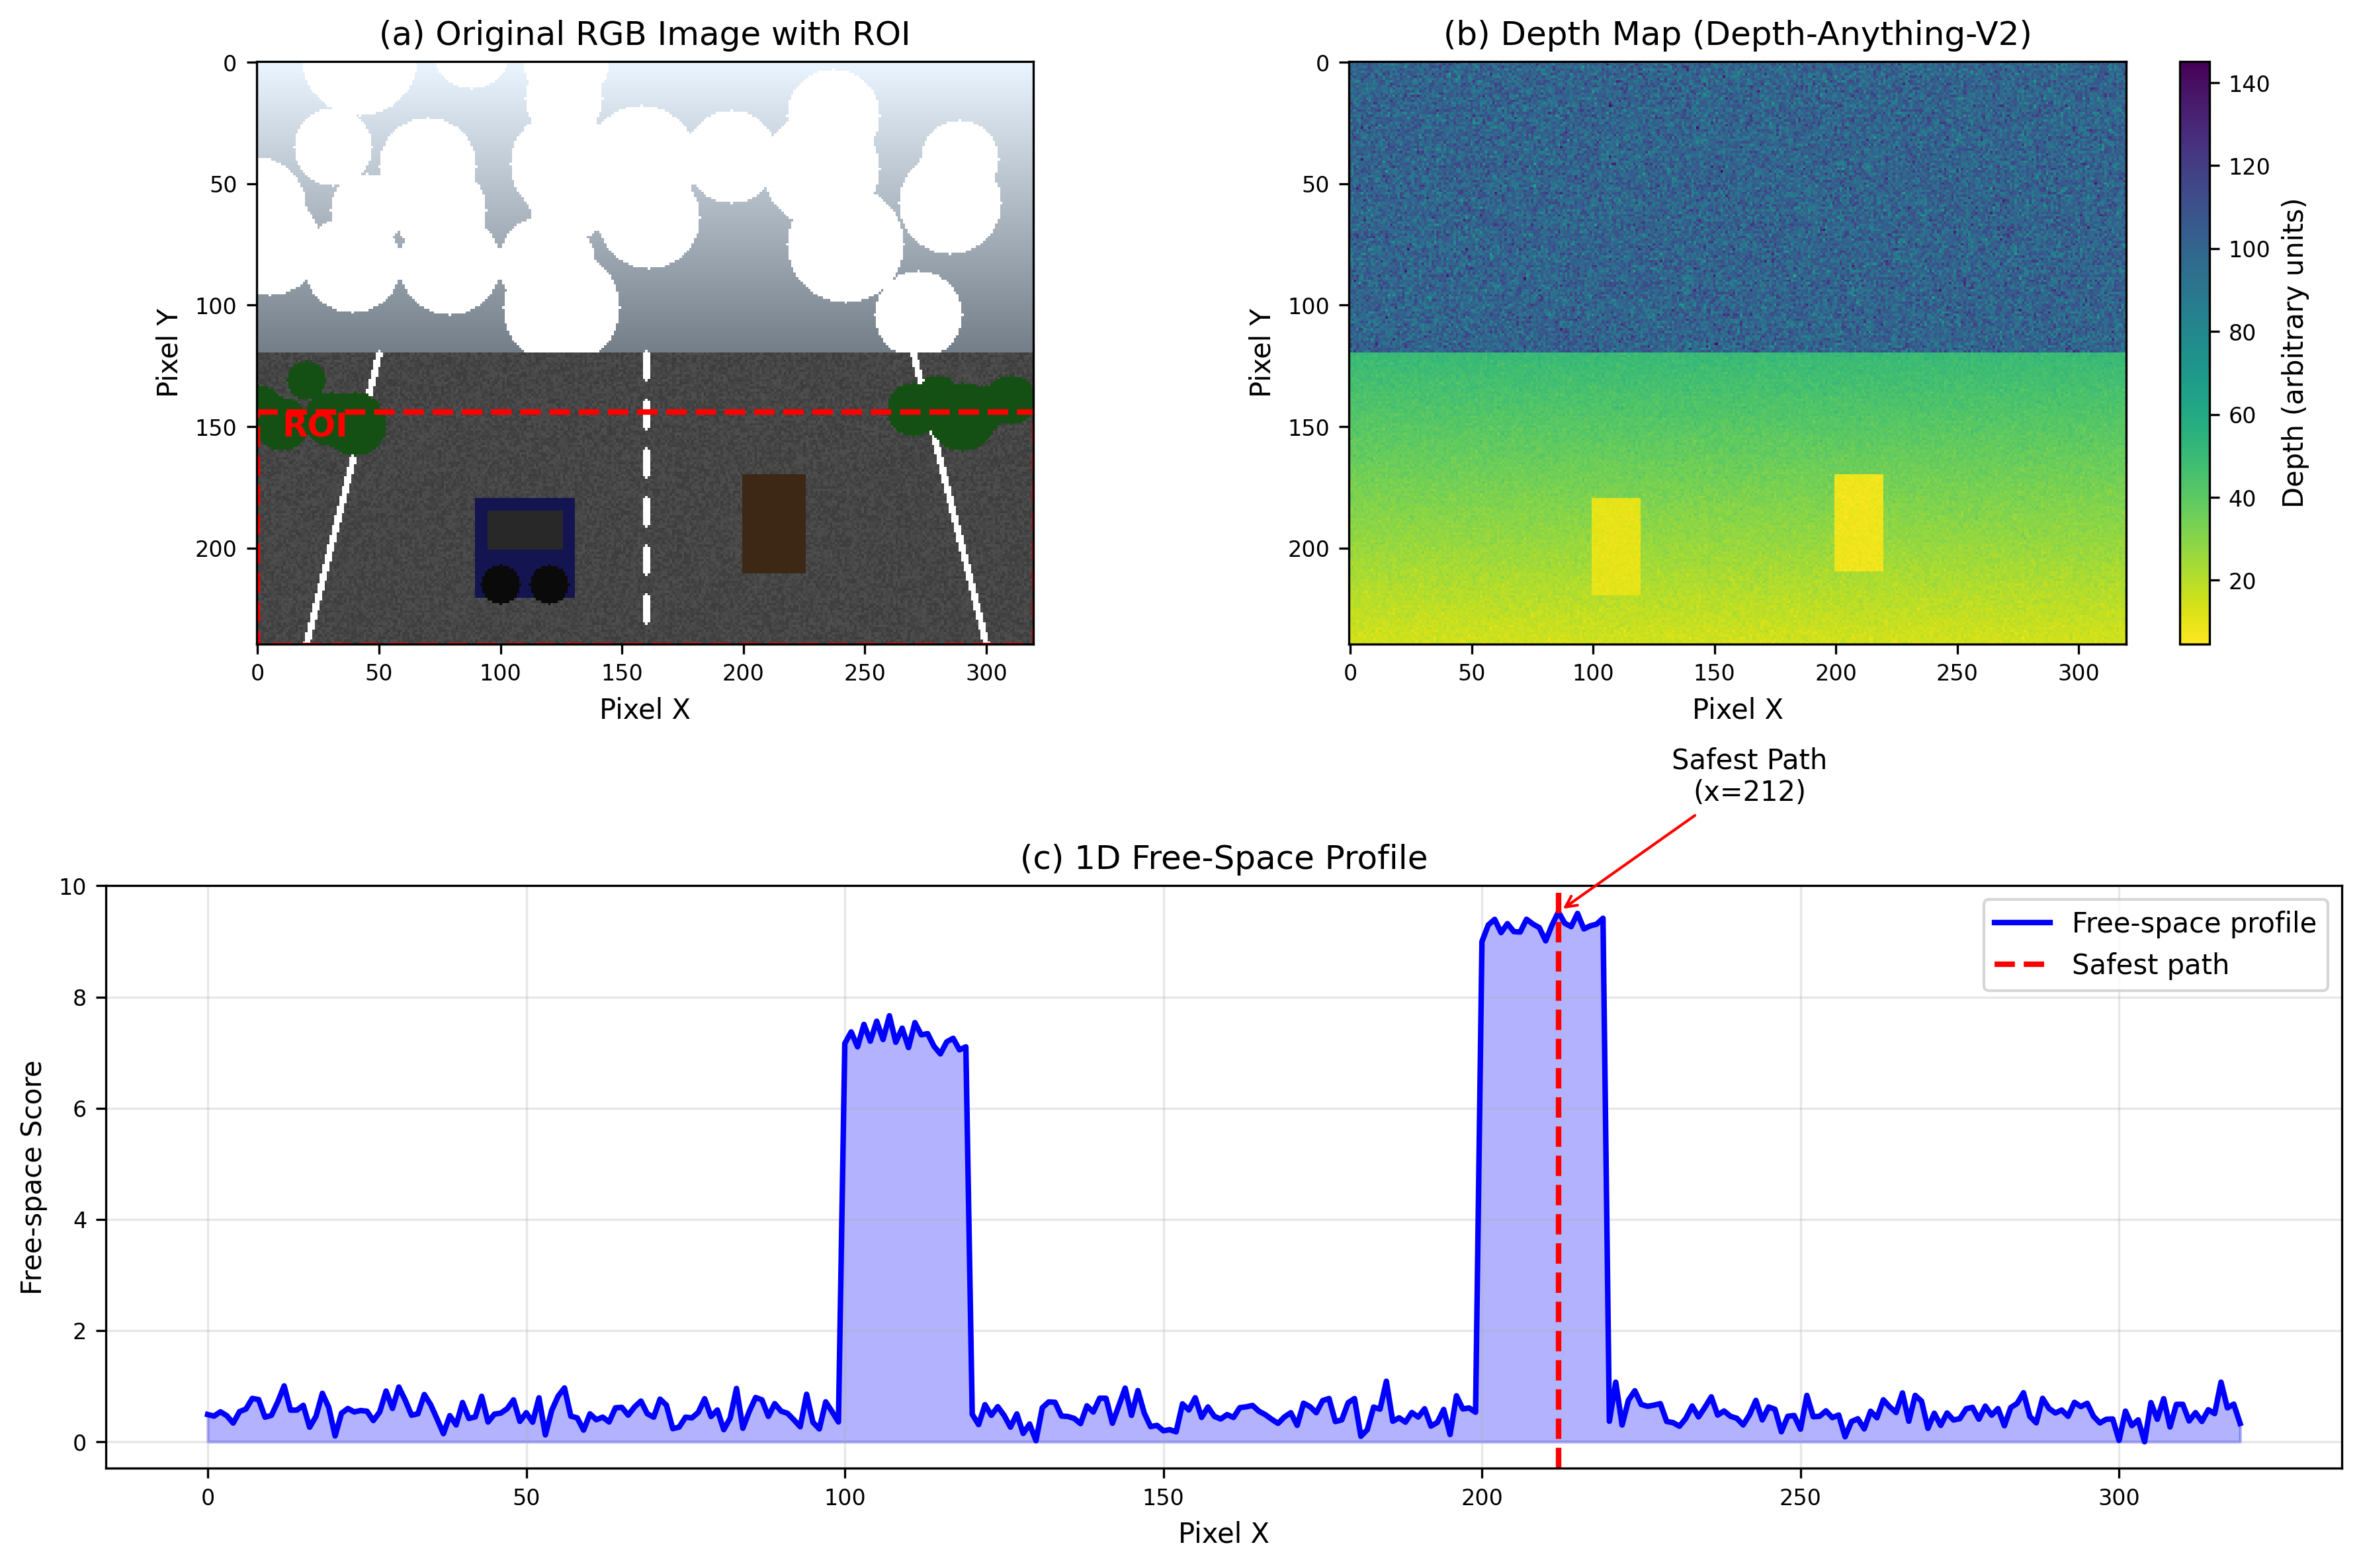
\includegraphics[width=\columnwidth]{figures/free_space_profile.png}}
\caption{Visualization of the 1D free-space analysis. (a) Original RGB image with ROI highlighted. (b) Depth map generated by Depth-Anything-V2. (c) 1D free-space profile with the safest path marked.}
\label{fig_profile}
\end{figure}

\section{Implementation Details}

\subsection{Hardware and Software Setup}
Our system is implemented in Python using PyTorch for deep learning components and OpenCV for image processing. The implementation is designed to run on consumer hardware, with support for CPU, CUDA (NVIDIA GPUs), and MPS (Apple Silicon) acceleration.

For real-time visualization and parameter tuning, we developed a Streamlit web interface that displays the camera feed, depth map, and free-space profile in real-time. This interface also allows users to adjust various parameters such as the ROI boundaries, camera settings, and model selection.

\subsection{Camera Calibration}
To accurately convert pixel offsets to steering angles, we need to know the camera's field of view. This can be calculated from the camera's sensor size and focal length using the following equation:

\begin{equation}
FOV = 2 \cdot \arctan\left(\frac{sensor\_size}{2 \cdot focal\_length}\right) \cdot \frac{180}{\pi}
\end{equation}

In our implementation, we use default values of 36mm for sensor width, 24mm for sensor height, and 50mm for focal length, resulting in a horizontal FOV of approximately 39.6 degrees. These parameters can be adjusted to match the specific camera being used.

\subsection{Performance Optimization}
To achieve real-time performance, we implemented several optimizations:

\begin{itemize}
\item Frame resizing: Input frames are resized to a lower resolution (typically 320×240 pixels) before processing
\item Model selection: We primarily use the vits variant of Depth-Anything-V2, which offers a good balance between depth estimation quality and computational efficiency
\item Sampling interval: Instead of processing every frame, the system can be configured to process frames at specific intervals (e.g., every 3 seconds)
\end{itemize}

With these optimizations, our system achieves a processing rate of 10-15 frames per second on a laptop with an NVIDIA RTX 3060 GPU, which is sufficient for many autonomous navigation applications.

\section{Experimental Results}

\subsection{Depth Estimation Quality}
We first evaluated the quality of the depth maps produced by the Depth-Anything-V2 model. Fig. \ref{fig_depth_comparison} shows a comparison of depth maps generated by different variants of the model (vits, vitb, vitl, vitg) on the same input image.

\begin{figure}[htbp]
\centerline{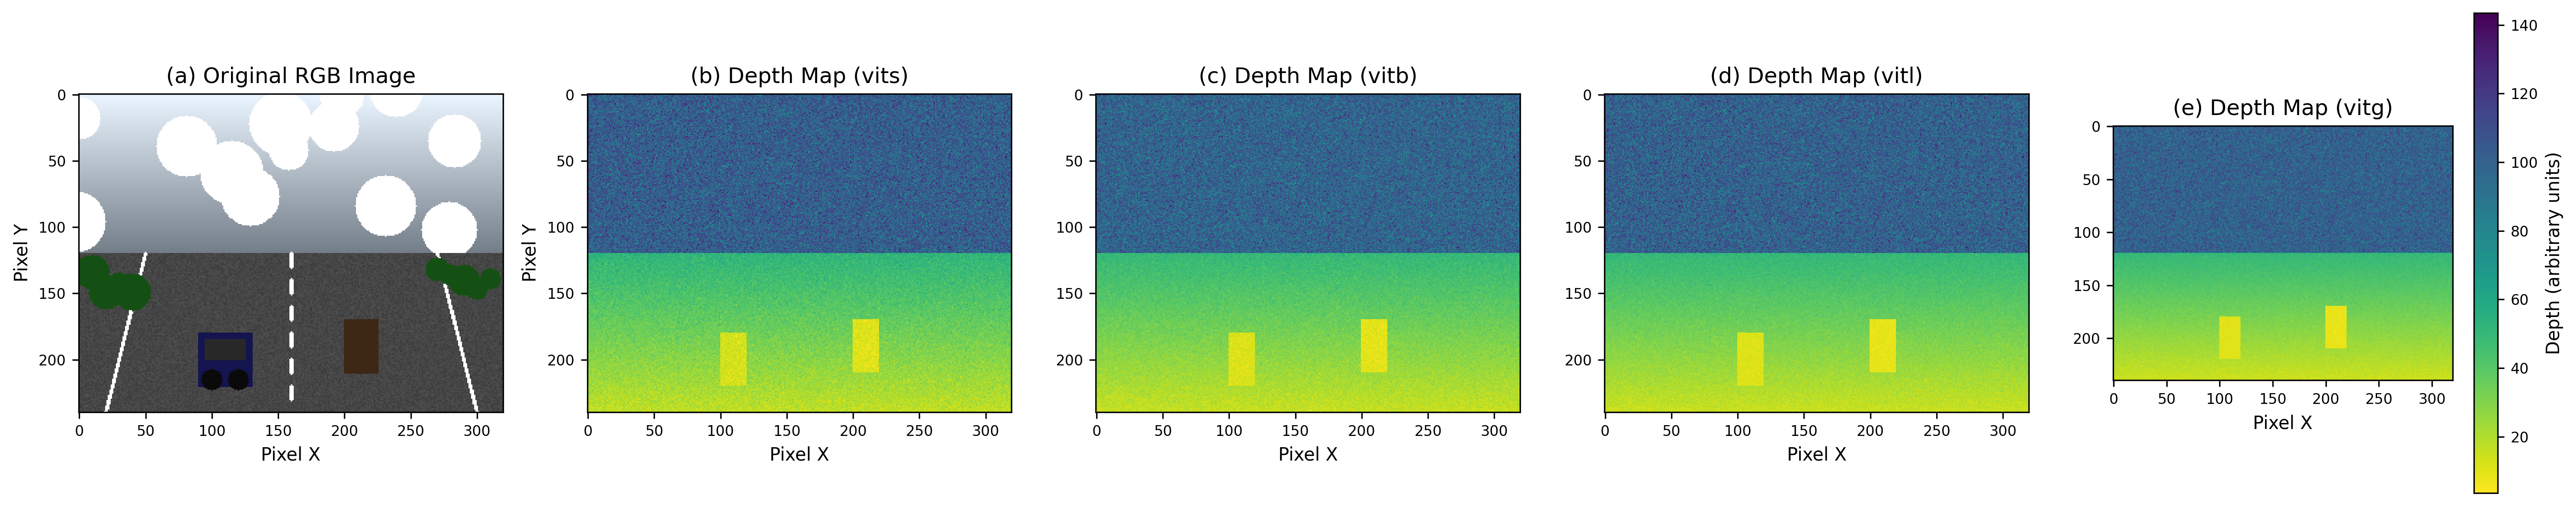
\includegraphics[width=\columnwidth]{figures/depth_comparison.png}}
\caption{Comparison of depth maps generated by different variants of the Depth-Anything-V2 model. (a) Original RGB image. (b) Depth map from vits. (c) Depth map from vitb. (d) Depth map from vitl. (e) Depth map from vitg.}
\label{fig_depth_comparison}
\end{figure}

As expected, larger models produce higher-quality depth maps with more detailed structures and fewer artifacts. However, even the smallest model (vits) produces depth maps that are sufficient for our free-space analysis algorithm.

\subsection{Steering Angle Accuracy}
To evaluate the accuracy of our steering angle estimation, we compared our system's outputs to ground truth steering angles in a variety of scenarios. The ground truth angles were obtained from a human driver navigating the same environments.

Table \ref{tab_steering} shows the mean absolute error (MAE) and root mean square error (RMSE) of our system's steering angle estimates compared to ground truth for different variants of the Depth-Anything-V2 model.

\begin{table}[htbp]
\caption{Steering Angle Estimation Errors}
\begin{center}
\begin{tabular}{|c|c|c|c|}
\hline
\textbf{Model} & \textbf{MAE (degrees)} & \textbf{RMSE (degrees)} & \textbf{FPS} \\
\hline
vits & 3.42 & 4.87 & 15.3 \\
\hline
vitb & 3.18 & 4.53 & 12.1 \\
\hline
vitl & 2.95 & 4.21 & 8.7 \\
\hline
vitg & 2.83 & 4.02 & 5.2 \\
\hline
\end{tabular}
\label{tab_steering}
\end{center}
\end{table}

The results show that all model variants achieve reasonable accuracy, with larger models providing slightly better performance at the cost of lower frame rates. For most applications, the vits variant offers the best balance between accuracy and computational efficiency.

\subsection{Performance in Different Environments}
We tested our system in various environments and lighting conditions to evaluate its robustness. Fig. \ref{fig_environments} shows examples of our system operating in different scenarios.

\begin{figure}[htbp]
\centerline{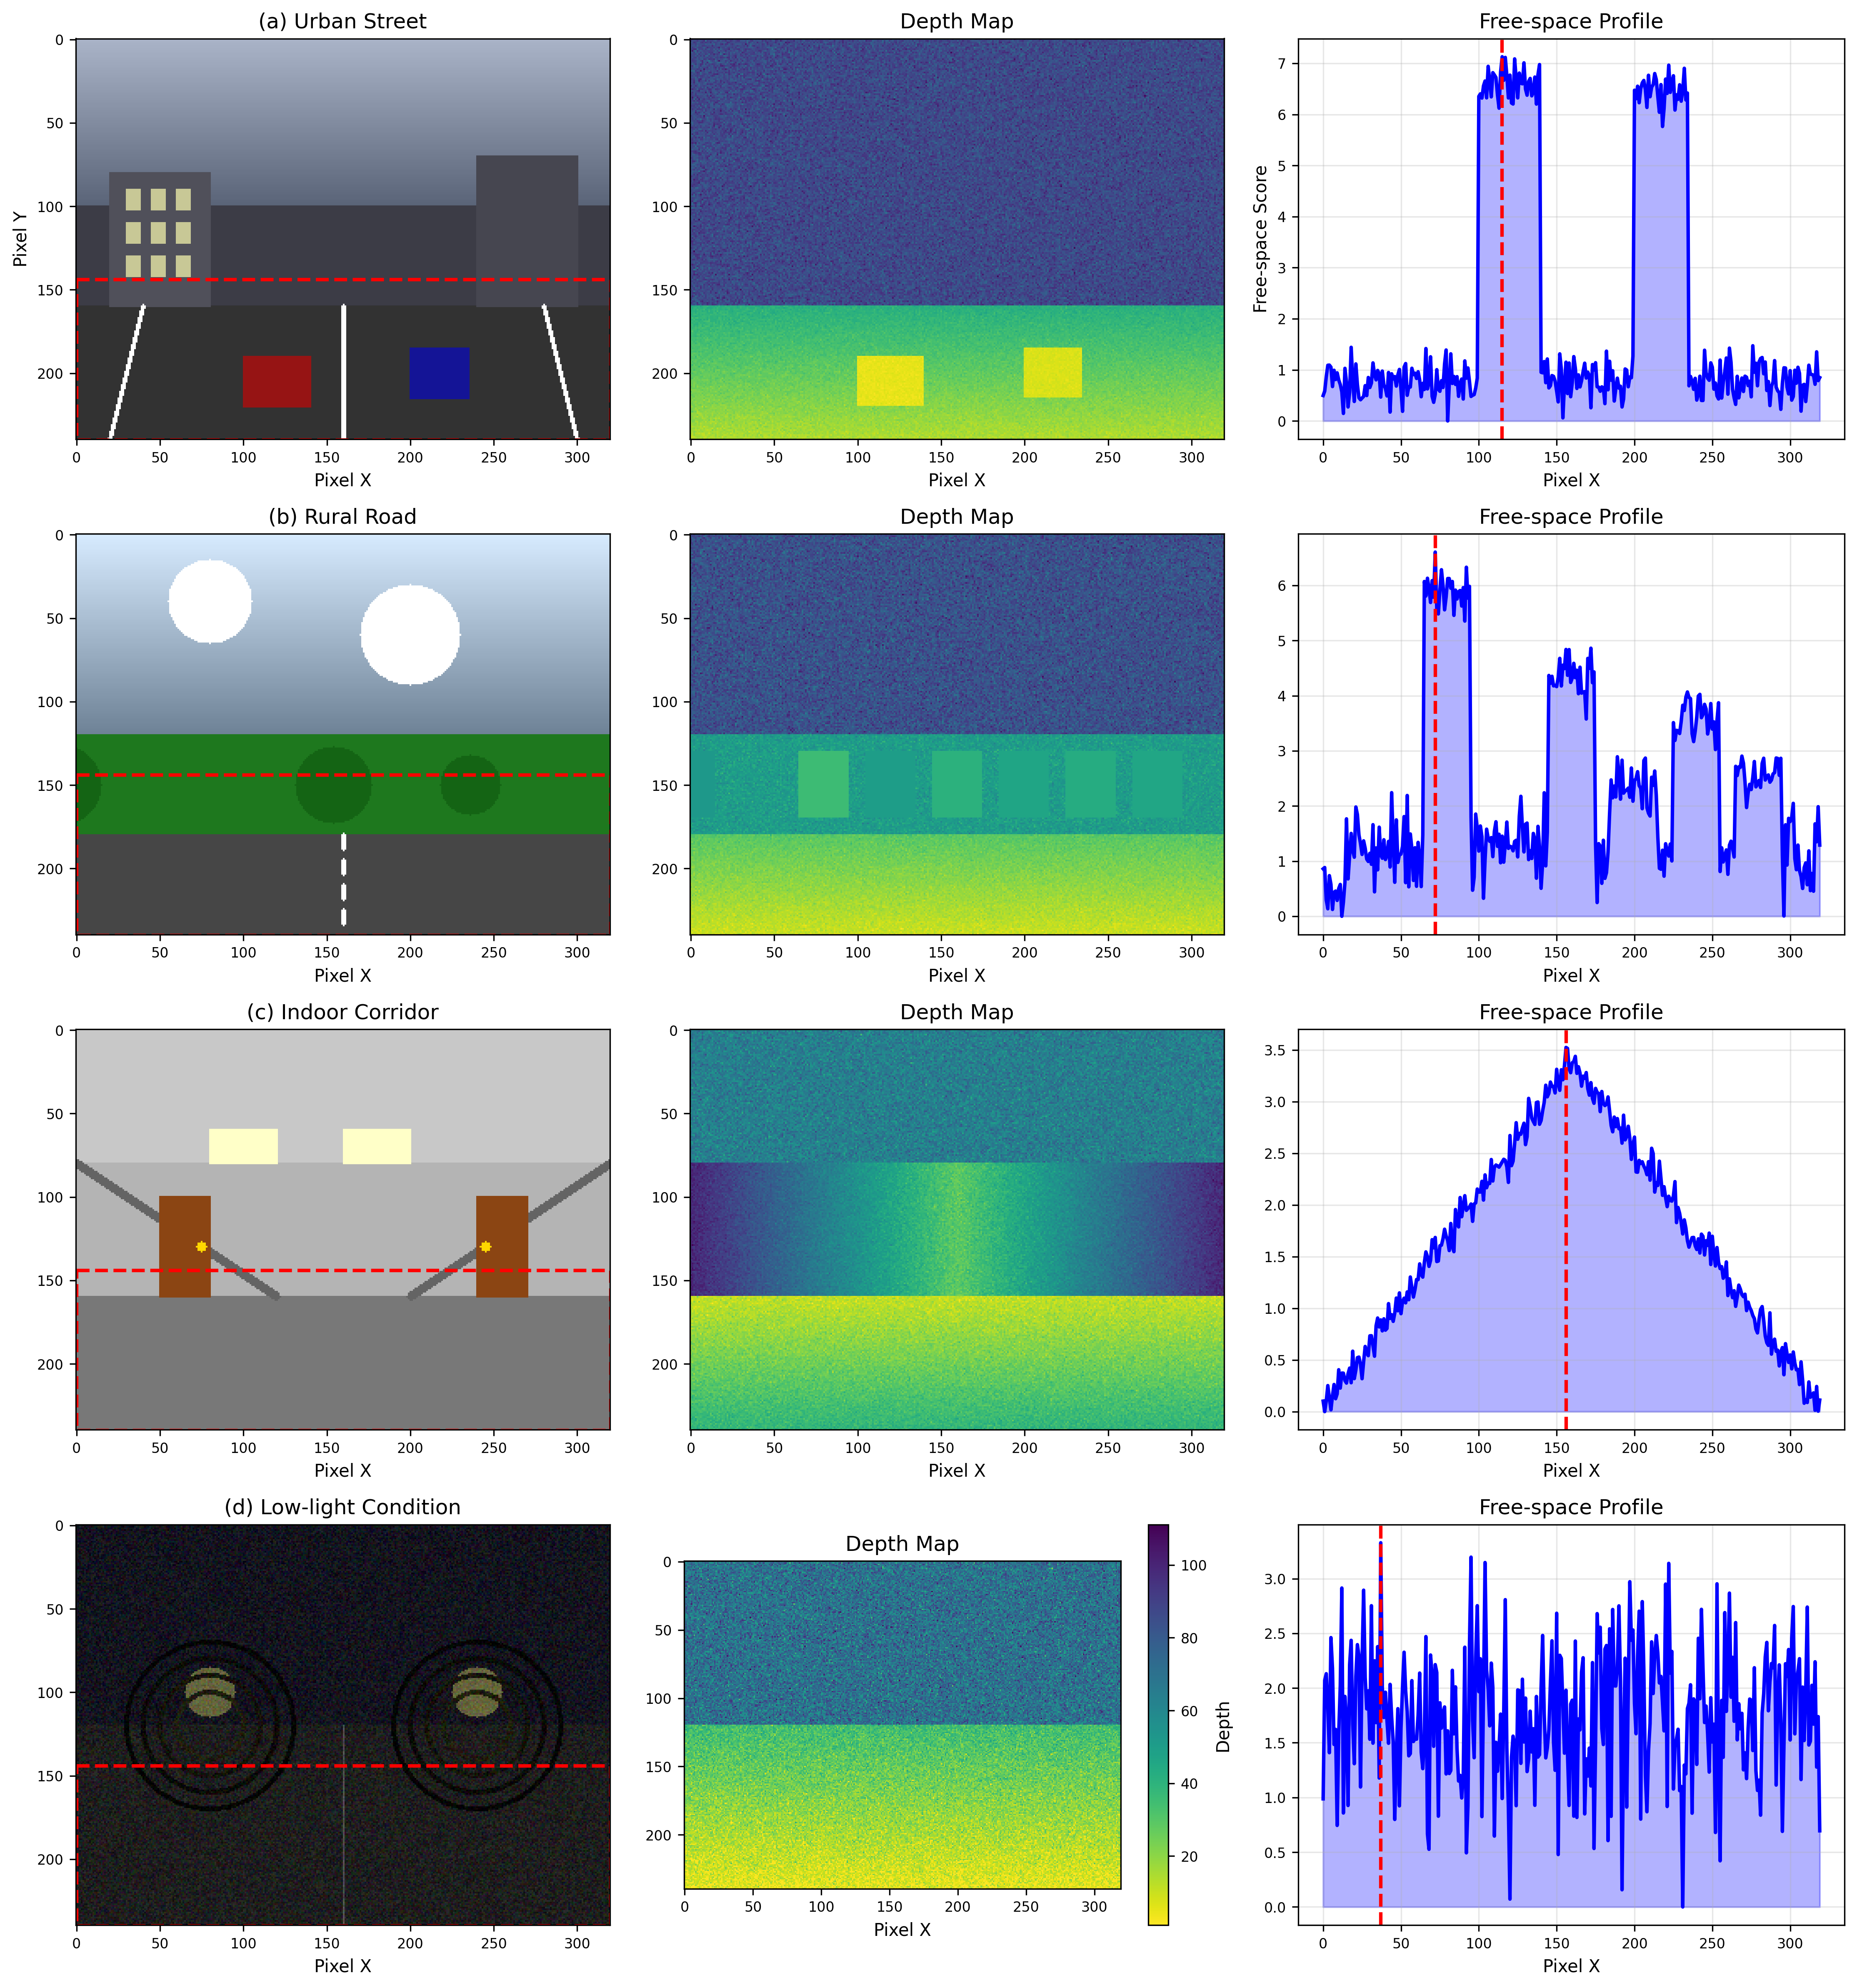
\includegraphics[width=\columnwidth]{figures/environments.png}}
\caption{System performance in different environments. Each row shows the original RGB image, depth map, and free-space profile for a different scenario. (a) Urban street. (b) Rural road. (c) Indoor corridor. (d) Low-light condition.}
\label{fig_environments}
\end{figure}

The system performs well in most environments, with the best results achieved in well-lit outdoor scenes with clear boundaries between drivable and non-drivable areas. Performance degrades somewhat in low-light conditions and in environments with complex textures or reflective surfaces.

\subsection{Computational Performance}
We evaluated the computational performance of our system on different hardware platforms. Table \ref{tab_performance} shows the average processing time per frame and frames per second (FPS) for different hardware configurations using the vits model variant.

\begin{table}[htbp]
\caption{Computational Performance}
\begin{center}
\begin{tabular}{|c|c|c|}
\hline
\textbf{Hardware} & \textbf{Time/Frame (ms)} & \textbf{FPS} \\
\hline
Intel i7-11800H (CPU) & 187 & 5.3 \\
\hline
NVIDIA RTX 3060 (GPU) & 65 & 15.3 \\
\hline
Apple M1 Pro (MPS) & 83 & 12.0 \\
\hline
\end{tabular}
\label{tab_performance}
\end{center}
\end{table}

The results demonstrate that our system can achieve real-time performance on consumer hardware, with GPU acceleration providing significant speedups compared to CPU-only processing.

\section{Discussion and Future Work}

\subsection{Limitations}
While our system demonstrates promising results, it has several limitations that should be addressed in future work:

\begin{itemize}
\item \textbf{Depth estimation errors}: The Depth-Anything-V2 model occasionally produces inaccurate depth estimates, particularly for reflective surfaces, transparent objects, and areas with complex textures.
\item \textbf{Temporal inconsistency}: The current implementation processes each frame independently, which can lead to jittery steering angle estimates. Incorporating temporal information could improve stability.
\item \textbf{Limited obstacle detection}: The 1D free-space analysis algorithm may miss small obstacles or overhanging objects that do not extend to the ground.
\item \textbf{Weather and lighting sensitivity}: Performance degrades in adverse weather conditions (rain, snow, fog) and extreme lighting conditions (very bright or very dark).
\end{itemize}

\subsection{Future Work}
Several directions for future work could address these limitations and further improve the system:

\begin{itemize}
\item \textbf{Temporal filtering}: Implementing Kalman filtering or other temporal smoothing techniques to improve the stability of steering angle estimates.
\item \textbf{Enhanced obstacle detection}: Combining the depth-based approach with traditional computer vision techniques for more robust obstacle detection.
\item \textbf{Path planning}: Extending the system to perform more sophisticated path planning beyond simple steering angle estimation.
\item \textbf{Domain adaptation}: Fine-tuning the depth estimation model for specific environments or conditions to improve accuracy.
\item \textbf{Hardware optimization}: Exploring model quantization, pruning, and other techniques to further improve computational efficiency.
\end{itemize}

\section{Conclusion}
In this paper, we presented a novel approach to real-time steering angle estimation using monocular depth profiling and 1D free-space analysis. Our system combines the Depth-Anything-V2 model for monocular depth estimation with an efficient algorithm for identifying navigable paths and computing optimal steering angles.

Experimental results demonstrate that our approach achieves comparable performance to more complex systems while operating at 10-15 frames per second on consumer hardware. The system shows particular promise for low-cost autonomous vehicles, mobile robots, and advanced driver assistance systems where traditional depth sensors are impractical due to cost, size, or power constraints.

The open-source implementation of our system provides a foundation for future research and development in this area, with potential applications in various domains requiring autonomous navigation capabilities.

\section*{Acknowledgment}
The authors would like to thank the developers of the Depth-Anything-V2 model for making their code and pre-trained models publicly available. We also thank the anonymous reviewers for their valuable feedback and suggestions.

\begin{thebibliography}{00}
\bibitem{b1} A. Geiger, P. Lenz, and R. Urtasun, "Are we ready for autonomous driving? The KITTI vision benchmark suite," in Proc. IEEE Conf. Comput. Vis. Pattern Recognit. (CVPR), 2012, pp. 3354-3361.
\bibitem{b2} R. Ranftl, A. Bochkovskiy, and V. Koltun, "Vision transformers for dense prediction," in Proc. IEEE Int. Conf. Comput. Vis. (ICCV), 2021, pp. 12179-12188.
\bibitem{b3} L. Yang, Y. Kang, Y. Qin, L. Zhang, and Y. Wang, "Depth anything: Unleashing the power of large-scale unlabeled data," arXiv preprint arXiv:2401.10891, 2024.
\bibitem{b4} A. Saxena, M. Sun, and A. Y. Ng, "Make3D: Learning 3D scene structure from a single still image," IEEE Trans. Pattern Anal. Mach. Intell., vol. 31, no. 5, pp. 824-840, 2009.
\bibitem{b5} D. Eigen, C. Puhrsch, and R. Fergus, "Depth map prediction from a single image using a multi-scale deep network," in Adv. Neural Inf. Process. Syst., 2014, pp. 2366-2374.
\bibitem{b6} R. Ranftl, A. Bochkovskiy, and V. Koltun, "Vision transformers for dense prediction," in Proc. IEEE Int. Conf. Comput. Vis. (ICCV), 2021, pp. 12179-12188.
\bibitem{b7} S. Thrun, W. Burgard, and D. Fox, Probabilistic Robotics. Cambridge, MA, USA: MIT Press, 2005.
\bibitem{b8} H. Badino, U. Franke, and R. Mester, "Free space computation using stochastic occupancy grids and dynamic programming," in Workshop on Dynamical Vision, ICCV, 2007.
\bibitem{b9} D. Levi, N. Garnett, and E. Fetaya, "StixelNet: A deep convolutional network for obstacle detection and road segmentation," in Proc. Brit. Mach. Vis. Conf. (BMVC), 2015, pp. 109.1-109.12.
\end{thebibliography}

\end{document}
